\section{Zielsetzung}

	In diesem Versuch werden allgemeine theoretische Begriffe in Verbindung mit Vakua erläutert.
	Experimentiell wird das Saugvermögen einer Drehschieberpumpe und einer Turbomolekularpumpe bestimmt.
	Dazu werden jeweils einige Evakurierungskurven aufgenommen und Leckratenmessungen durchgeführt.

\section{Theorie}
	
	\subsection{Vakuum}
		
		Allgemein wird von einem Vakuum gesprochen, sobald der Druck innerhalb eines Gefäßes niedriger als sein Umgebungsdruck ist.\\
		Da der niedrigste auf der Erde vorkommende Atmosphärendruck in großer Höhe bei $p = \SI{300}{\milli\bar}$ liegt, wird ab dann von einem Vakuum gesprochen.\\
		Es ist in diesem Versuch eine gute Annäherung wenn wir bei dem vorliegendem Gas von idealem Gas sprechen. 
		Dies bedeutet, dass jegliche Wechselwirkungen zwischen Teilchen nur durch vollkommen elastische Stöße passieren und die Gasteilchen keine Ausdehnung besitzen.\\
		Wenn dies angenommen wird, kann das Gas auch mit der Idealen Gasgleichung
		\begin{equation}
			p \cdot V = N \cdot \symup k _{\symup b} \cdot T
		\end{equation}
		beschrieben werden.
		Hier ist $p$ der Druck, $V$ das Volumen, $N$ die Teilchenzahl, $\symup k _{\symup b}$ die Boltzmann Konstante und $T$ die Temperatur. 
		Ein Spezialfall dieser Gleichung ist das \textit{Gesetz von Boyle-Mariotte}. Dieses besagt, dass bei konstanter Temperatur
		\begin{equation}
			p \propto V^{-1}
		\end{equation}
		ist.

	\subsection{Fachbegriffe}

		\subsubsection{mittlere freie Weglänge}
			\noindent
			Die mittlere freie Weglänge beschreibt die durschnittliche Fluglänge eines Gasteilchens zwischen zwei Kollisonen mit anderen Gasteilchen.\\
			(Quelle: \cite{wiki:mfg})

		\subsubsection{Sorption}
			
			\noindent
			Die Sorption bezeichnet den Vorgang einer Anreicherung eines Stoffes. 
			Hier beschreibt die Absorption, wenn der Stoff innerhalb einer Phase aufgenommen wird. Ein Beispiel ist die Aufnahme einer Elektromagnetischenwelle.\\
			Adsorption ist im Gegensatz zur Absortion die Anlagerung auf der Oberfläche oder Grenzfläche eines Stoffes.\\
			Die \textit{Desorption} beschreibt gegensätzlich einen Prozess bei dem Atome oder Moleküle die Oberfläche eines Festkörpers verlassen und in die Gasphase übergehen.\\
			(Quelle: \cite{wiki:sorp})
			
		\subsubsection{Lecks}

			Lecks beschreiben Prozesse die das Vakuum reduzieren. Es wird dabei zwischen realen und virtuellen Lecks unterschieden.\\
			Reale Lecks sind Prozesse die von außerhalb der Vakuumanlage messbar sind. Eine nicht korrekt verschlossene Verbindung ist zum Beispiel ein reales Leck.\\
			Virtuelle Lecks entstehen zum Beipiel durch Einschlüsse in der Vakuumanlage, welche sich mit zunehmendem Druck freisetzten.
			Diese Art von Lecks sind von außen nicht zu messen und müssen beim Aufbau oder in der Produktion der Teile verhindert werden.\\
			(Quelle: \cite{pfeiffer:grund})

	\subsection{Vakuumbereiche}

			\noindent
		Physikalisch sind mehrere Vakuumbereiche definiert, da die verschiedenen Dichten zu stark unterschiedlichem Gasverhalten führen. 

		\subsubsection{Grobvakuum}
			\noindent
			Im ersten relevanten Druckbereich wird von einem Grobvakuum gesprochen. Dieses ist zwischen $\SI{300}{\milli\bar}$ und $\SI{1}{\milli\bar}$ definiert.\\
			In diesem Bereich findet allgemein viskose Strömung statt, in der der Großteil der Stöße zwischen den Gasteilchen untereinander und nicht mit der Gefäßwand stattfinden.\\
			Es muss jedoch abhängig von der Teilchengeschwindigkeit, der Teilchendichte und der Gefäßgröße zwischen laminarer oder turbolenter Strömung unterschieden. 
			%hier könnten noch Formeln und weitere Informationen zu den Strömungsarten eingefögt werden

		\subsubsection{Feinvakuum}

			\noindent
			Das Feinvakuum ist zwischen $\SI{1}{\milli\bar}$ und $\SI{e-3}{\milli\bar}$ definiert. Hier findet Knudsen-Strömung statt.

			\noindent
		\subsubsection{Hoch und Ultrahochvakuum} 
			Es wird ab einem Druck von $\SI{e-3}{\milli\bar}$ bis $\SI{e-8}{\milli\bar}$ von Hochvakuum gesprochen. Von Ultrahochvakuum ist ab $\SI{e-8}{\milli\bar}$ die Rede.	\\	
			In diesen beiden Druckbereichen findet nur noch Molekulare-Strömung statt.\\
			Dies bedeutet, dass die Teilchen untereinander fast nicht mehr Wechselwirken. Mathematisch ist hier die mittlere freie Weglänge größer als die Weite des Strömungskanals.
		\\
		\\
		Diese unterschiedlichen Strömungsarten haben hohe Relevanz bei praktischen Anwendungen, da zum Beispiel das effektive Saugvermögen von Vakuumpumpen beeinträchtigt werden kann.\\
		Im Grobvakuum ist es wichtig einen großen Leitungsdurchmesser einzubauen, damit laminare Stömung sicher gestellt ist.
		Im Ultrahochvakuum reichen relativ kleine Leitungsdurchmesser jedoch wieder aus.\\
		(Quelle: \cite{pfeiffer:grund})

	\subsection{Arten der Vakuumerzeugung}	
		
		\noindent
		Vakuumpumpen können sich stark in ihrer Funktionsweise abhängig vom Arbeitsbereich unterscheiden.\\	
		Der größte Unterschied liegt zwischen gasbindenden und gasfördenden Vakuumpumpen, wobei sich gasfördernde Pumpen noch einmal in verdrängende und kinetische Pumpen unterteilen.\\
		Gasbindende Vakuumpumpen funktionieren durch Sorption, indem Gasteilchen von der Pumpe aufgenommen werden. 
		Dieses Prinzip ergibt erst bei bereits sehr gutem Vakuum Sinn.  \\
		Gasfördernde Vakuum fördern Gas durch abgeschlossene Volumina, welche komprimiert werden oder sich ausdehnen.\\
		Kinetische Pumpen erhöhen das Vakuum, indem Gasteilchen in Richtung der Pumprichtung beschleunigt werden.
		Auch dieses Vakuumerzeugungsprinzip hat bei Atmosphärendruck einige Probleme und benötigt ein Vorvakuum.

		\subsubsection{Drehschiebervakuumpumpe} 
						
			\begin{figure}
				\centering
				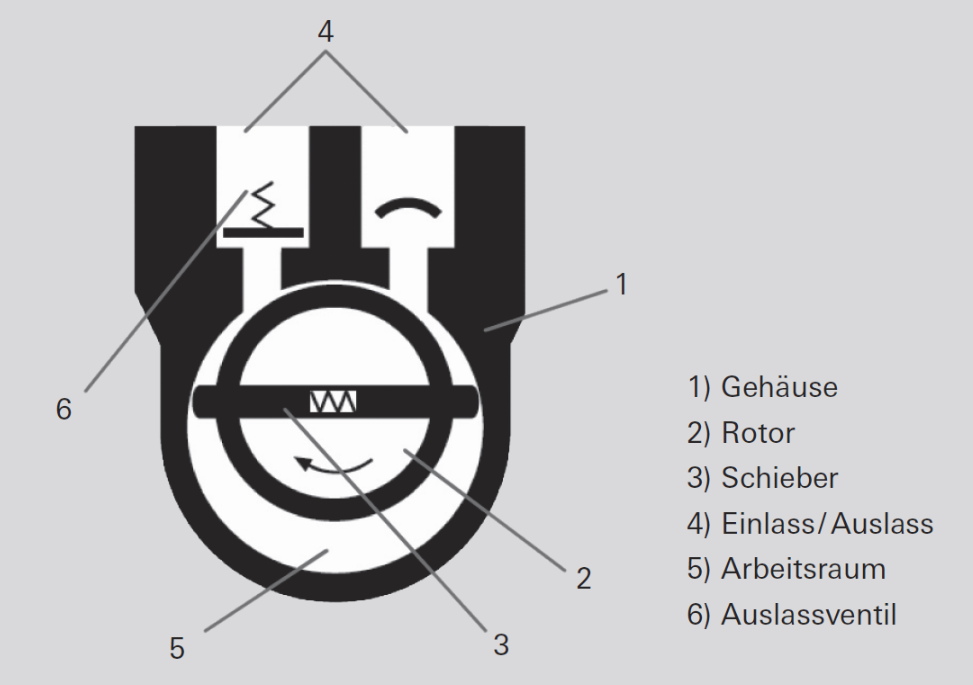
\includegraphics[width=0.5\linewidth]{"latex/images/Drehschieber.png"}
				\caption{Der schematische Aufbau einer Drehschiebervakuumpumpe. \protect Quelle: \cite{pfeiffer:pump}}
				\label{fig:dreh}
			\end{figure}  

			\noindent
			Die Drehschieberpumpe ist eine Rotationsverdrängerpumpe.	
			besteht aus dem Gehäuse (1), dem eingebauten Rotor(2), den mit Flieh- und Federkraft radial bewegten Schiebern(3) und dem Ein- bzw. Auslass(4).\\ 
			Das Innere des Arbeitsraumes(5) wird durch den Stator, den Rotor und die Schieber in mehrere Bereiche eingeteilt. 
			Diese saugen beim Drehen neues Gas aus dem Rezipienten und erhöhen dessen Vakuum, wenn sie expandieren.
			Sobald das Volumen dann wieder vom Rezipienten getrennt ist, wird es komprimiert, um dann Gas durch den Auslass zu drücken.\\
			Eine zweistufige Drehschieberpumpe kann Drücke bis zu $\SI{5e-4}{\milli\bar}$ erreichen. \\
			In diesem Versuch wird jedoch nur eine einstufige Pumpe mit einem Enddruck von $p = \SI{2.1 e-2}{\milli\bar}$ genutzt.\\
			Ein Nachteil der Drehschieberpumpe ist, dass unter anderem zum Abschließen der Kammern, Öl verwendet wird.
			Mittels Desorption können daher Moleküle aus dem Öl in das Gas übergehen und dieses verunreinigen.	 

		\subsubsection{Turbomolekularpumpe}
		
			\noindent
			Turbomolekularpumpen sind turbinenähnliche kinetische Vakuumpumpen.\\ 
			In ihrem Gehäuse ist ein mehrstufiger Rotor mit Schaufeln.
			Zwischen den Rotorscheiben sind beschaufelte Statorscheiben mit spiegelverkehrter Symmetrie zu den Rotorscheiben.\\
			Die Rotorscheiben drehen sich nun mit bis zu $\SI{1500}{\hertz}$, damit die Schaufeln eine Rotationsgeschwindigkeit ähnlich der mittleren Teilchengeschwindigkeit haben. \\
			Durch Wechselwirkung mit den Rotor und Statorschaufeln werden die Gasteilchen in Pumprichtung beschleunigt.
			Eine Voraussetzung für diese Funktionsweise ist, dass in der Pumpe Molekulare-Strömung vorliegt.\\ 
			Die mittlere freie Weglänge muss größer sein, als die Abstände zwischen Rotor und Statorscheiben, damit die Teilchen ihre Bewegungsrichtung bei behalten.\\
			(Quelle: \cite{pfeiffer:pump})
			  					
	\subsection{Saugvermögen}

			\noindent
		Im Allgemeinen beschreibt das Saugvermögen $S$ einer Vakuumpumpe, wie viel Gas sie aus dem Rezipienten ziehen kann. 
		\begin{equation}
			S = \frac{\text{d}V}{\text{d}t}
		\end{equation}
		Um dieses zu Bestimmen werden in diesem Versuch Evakuierungskurven, also der Druck innerhalb des Rezipienten augenommen, und Leckratenmessungen durchgeführt.

		\subsubsection{Messung der p(t)-Kurve}
			
			\noindent
			Wird die Gleichung:
			\begin{equation}
				p \cdot V = \text{const}
			\end{equation}
			nach der Zeit abgeleitet, entstehen auf der linken Seite zwei Summanden. \\
			Wird nun mit dem Druck $p$ multipliziert kann die Ableitung des Volumens als das Saugvermögen $S$ identifiziert werden.\\
			Durch Verschieben der Terme entsteht folgende Gleichung:
			\begin{equation}
				\frac{\text{d}V}{\text{d}t} = S = - \frac{V}{p} \frac{\text{d}p}{\text{d}t}
			\end{equation}
			Diese Differentialgleichung wird mittels einer Exponentialfunktion mit dem Saugvermögen $S$ dem Volumen $V$ und der Zeit $t$ im Exponenten gelöst:
			\begin{equation}
				p(t) = p_0 \text{exp}\left( - \frac{S}{V_0}t \right)
			\end{equation}
			Jedoch muss noch beachtet werden, dass alle Vakuumpumpen einen gewissen Enddruck $p_\text{E}$ haben. 
			Sobald dieser Druck erreicht ist kann die Pumpe den Druck nicht weiter erhöhen und es entsteht ein Gleichgewicht zwischen Saugvermögen und 
			vakuumreduzierenden Prozessen wie Desorption oder Lecks.\\
			Der Gleichgewichtsdruck wird in der Evakuierungskurve durch Verschieben und skalieren der Exponentialfunktion eingerechnet:
			\begin{equation}
				p(t) = (p_0 - p_\text{E}) \text{exp}\left( - \frac{S}{V_0}t \right) + p_\text{E}
				\label{eqn:druckkurve}
			\end{equation}
			Mit dieser Formel lässt sich aus der Evakuierungskurve eine Schätzung für das Saugvermögen einer Vakuumpumpe berechnen.
			Jedoch muss beim Auswerten darauf geachtet werden, dass Vakuumpumpen zum Beispiel in unterschiedlichen Strömungsarten, auch verschiedene Saugvermögen haben.
			
		\subsubsection{Leckratenmessung}
			
			\noindent
			Zur Berechnung des Saugvermögens mittels Leckratenmessung muss zunächst die Leckrate $Q$ mittels des Gleichgewichtsdruck $p_\text{g}$ definiert werden:
			\begin{equation}
				S = \frac{Q}{p_\text{g}},
			\end{equation}
			und
			\begin{equation}
				Q = V_0 \frac{\Delta p}{\Delta t}.
			\end{equation}
			Hieraus folgt nun wieder ein Ausdruck für das Saugvermögen der Vakuumpumpe:
			\begin{equation}
				S = \frac{V_0}{p_\text{g}} \cdot \frac{\Delta p}{\Delta t.}
			\end{equation}
		\subsubsection{Leitwert}

			\noindent
			Bei all diesen Berechnungen ist zu bedenken, dass das theoretische Saugvermögen $S_0$ immer durch die Vakuumanlage reduziert wird.
			Dieser Effekt wird durch den Leitwert des Rezipienten beschrieben. Er gibt den reziproken Strömungswiderstand der Schläuche und Verbindungen an.\\
			Das effektive Saugvermögen $S_\text{eff}$, dass tatsächlich am Rezipienten ankommt, berechnet sich damit zu:
			\begin{equation}
				S_\text{eff} = \frac{S_0 \cdot L}{S_0 + L}.
			\end{equation}

	\subsection{Arten der Vakuummessung}
		
		\subsubsection{Pirani-Vakuummeter}
			
			\noindent
			Das Pirani-Vakuummeter arbeitet optimal im Bereich des Feinvakuums.\\
			Es nutzt aus, dass in diesem Druckbereich die Wärmeleitfähigkeit proportional zum Druck ist. 
			Der Wärmetransport geschieht hier primär durch direkte Stöße von Gasteilchen untereinander. \\
			Die Messung erfolgt über einen Draht in dem Rezipienten, durch den ein konstanter Strom fließt.
			Nun kann mittels einer Wheatstone-Brücke der Widerstand dieses Leiters und somit die Temperatur des Drahtes bestimmt werden.\\
			Da der Draht sich abhängig von dem Druck im Rezipienten unterschiedlich schnell abkühlt, kann mit dieser Methode auch der Druck in dem Rezipienten bestimmt werden.

		\subsubsection{Penning-Vakuummeter}

			\noindent
			Das Penning-Vakuummeter ist ein Kalt-Ionisations-Vakuumeter.\\
			Es arbeitet im Hoch- und Ultrahochvakuum. 
			Es beruht darauf, dass durch ein elektrisches Feld Atome ionisiert werden.
			Die frei werdenden Elektronen werden beschleunigt und ionisieren auf ihrem Beschleunigungsweg weitere Atome.\\
			Diese Ionen werden dann zu der Kathode beschleunigt und erzeugen dort einen Strom, welcher ein Maß für das Vakuum ist.

		\subsubsection{Bayard-Alpert-Vakuummeter}

			\noindent
			Das Bayard-Alpert-Vakuummeter ist eine Heiß-Ionisations-Vakuumeter.\\ Es arbeitet sehr Analog zu dem Penning-Vakuumeter.
			Der einzige Unterschied ist, dass die Elektronen durch einen Glühdraht frei werden.
		
		\subsubsection{Piezo-Vakuummeter}
			
			\noindent
			Ein Piezo-Vakuumeter vermisst das Vakuum direkt, indem es die Kraft des Gases auf eine Oberfläche misst. \\
			Da mit immer besser werdendem Vakuum auch die Kraft abnimmt, eignet sich dieses Vakuummeter am besten bis zum Grobvakuum ($\SI{1000}{\milli\bar}$ bis $\SI{1}{\milli\bar}$).\\
			Die konkrete Messung erfolgt mittels Piezo-Kristallen, welche bei Kompression eine elektrische Spannung erzeugen, die dann abgelesen wird.\\
			Aufgrund der ähnlichen Arbeitsbereiche werden, wie auch in diesem Versuch, Piezo- und Pirani-Vakuummeter oft in einem Messgerät kombiniert.

			\newpage
